\documentclass[border=4pt]{standalone}
\usepackage{tikz}
\usetikzlibrary{arrows.meta,calc,shapes.multipart}
\begin{document}
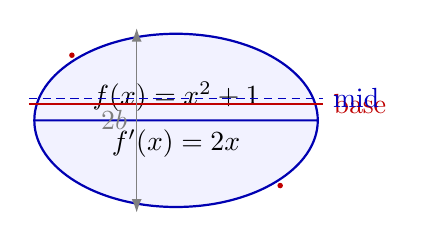
\begin{tikzpicture}[>=Latex]
  \node[ellipse split,draw=blue!70!black,thick,fill=blue!5,
    inner xsep=6pt,inner ysep=3pt,outer sep=2pt,
    minimum width=36mm,minimum height=22mm] (map)
    {$f(x)=x^2+1$\nodepart{lower}$f'(x)=2x$};

  \draw[red!75!black,thick] (map.base west) -- (map.base east)
    node[right] {base};
  \draw[blue!75!black,densely dashed] (map.mid west) -- (map.mid east)
    node[right] {mid};
  \draw[<->,gray] ($(map.south)+(-5mm,0)$) --
    node[left] {$2b$} ($(map.north)+(-5mm,0)$);
  \fill[red!75!black] (map.north west) circle (1pt)
    (map.south east) circle (1pt);
\end{tikzpicture}
\end{document}
